\model{Stack Diagrams}

Each method has its own area of memory to store parameters and other variables.
When a method is invoked, Java allocates this memory on the \emph{call stack}.
For convenience, we draw ``stack'' diagrams upside down.

\begin{center}

\includegraphics[height=3in]{stack-rings1.png}
\hspace{1em}
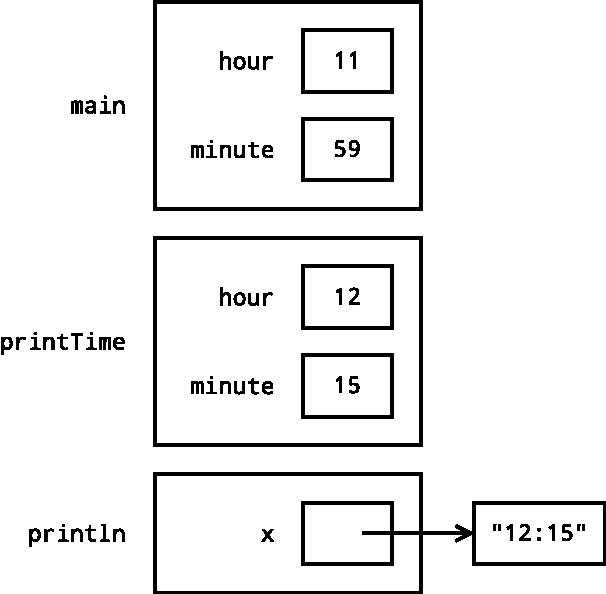
\includegraphics[height=3in]{stack1.pdf}
\end{center}

\begin{center}
Note: The signature for \java{System.out.println} is ~\java{public void println(String x)}.
\end{center}

\begin{javalst}
    public static void printTime(int hour, int minute) {
        System.out.println(hour + ":" + minute);
    }
    
    public static void main(String[] args) {
        int hour = 11;
        int minute = 59;
        printTime(12, 15);
    }
\end{javalst}


\quest{15 min}


\Q Based on the diagram, how many methods does the program call? \ans{Three}
\vspace{1ex}


\Q Based on the diagram, how many variables does the program have? \ans{Five}
\vspace{1ex}


\Q How do stack diagrams extend the memory diagrams we've seen previously?

\begin{answer}[5em]
There is a box for each method call, with the name of the method on the left.
Note that reference types (like strings) are not stored ``on the stack'' --- the variables are part of the method, but the actual data is outside of the method.
\end{answer}


\Q How is it possible that two variables with the same name can have different values?

\begin{answer}
Each method declares its own variables.
Because they are stored in different memory locations, the values are independent from other methods.
\end{answer}


\Q \label{drawing}
Draw a stack diagram to show the state of memory just before \java{println} is called.
Assume the user inputs the value 10.
(You should be able to do this kind of math without a calculator.)

\vspace{1ex}
\begin{javalst}
    public static void show(double c) {
        double f;
        String str;
        f = c * 1.8 + 32;
        str = String.format("%.1f C = %.1f F\n", c, f);
        System.out.println(str);
    }

    public static void main(String[] args) {
        double c;
        Scanner in = new Scanner(System.in);
        System.out.print("Enter temperature in Celsius: ");
        c = in.nextDouble();
        show(c);
    }
\end{javalst}
\vspace{-1ex}

\begin{answer}[3.1in]
\hfill
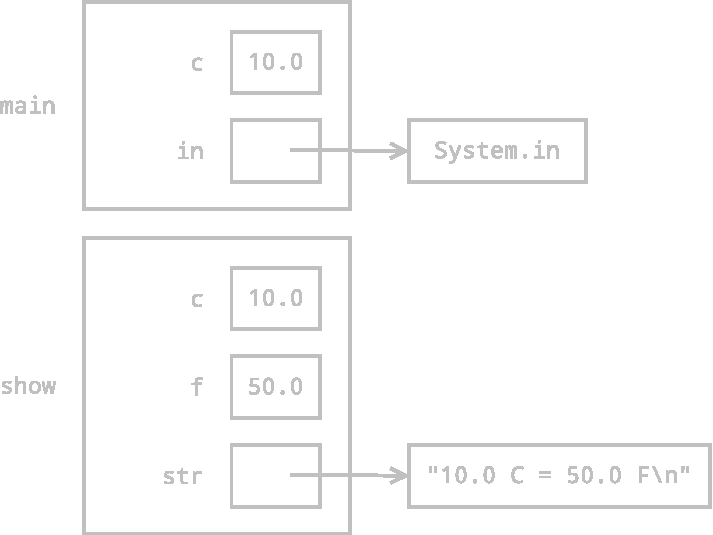
\includegraphics[height=3in]{stack2.pdf}
\end{answer}


\Q What is the difference between the \java{String.format} method (used in the previous question) and \java{System.out.printf}?

\begin{answer}
They both substitute values based on format specifiers.
\java{String.format} returns a new string, whereas \java{System.out.printf} displays it on the screen.
(In fact, \java{System.out.printf} invokes the \java{String.format} method.)
\end{answer}
